%% ============================================================================
%% ============================================================================
\section{The Bound and Its Application}
\label{sec:ident}

The estimator is pure accounting, with no run threshold and no fitted parameter. Let
$\phi$ be the fraction of reserves impaired, $\rho\in[0,1]$ the expected recovery rate on
the impaired assets, and $q\in[0,1]$ the probability under the pricing measure that the
loss on the impaired fraction goes unremediated. Expected backing per coin is
\begin{equation}
P_{\mathrm{fund}}(q,\rho) = 1 - q\,\phi\,(1-\rho),
\end{equation}
and its minimum over $q$ and $\rho$, the worst-case floor, is $1-\phi$. The estimator
rests on three assumptions, and a fourth serves the preference-free argument below.

\begin{description}
\item[(A1) Reserve-only fundamental.] A coin's fundamental value is its expected reserve
  backing per unit given disclosed reserves, and the only impairment is the
  exposure $\phi$.
\item[(A2) Par redemption when solvent.] Conditional on rescue, redemption is at \$1
  within the frozen window.
\item[(A3) Bounded recovery.] Recovery on impaired reserves satisfies $\rho\in[0,1]$,
  because the coin is fully reserved and the reserves carry no leverage.
\item[(A4) Monotone-utility valuation.] The unconstrained marginal holder values the claim
  as an expected utility of its payoff, for some monotone increasing utility and some
  probability measure over outcomes, with no ambiguity about the disclosed $\phi$. This nests risk neutrality, any degree of risk
  aversion, and rank-dependent weighting.
\end{description}

\begin{proposition}[Rational-pricing floor and impossibility]
\label{prop:floor}
Assume \textup{(A1)--(A3)}. Then
$P_{\mathrm{fund}}(q,\rho)\in[\,1-\phi,\,1\,]$ for all $q,\rho\in[0,1]$, so no expected
loss on the disclosed impairment justifies a value below $1-\phi$. The unremediated-loss
probability an observed price $P_{\mathrm{obs}}<1-\phi$ would require, at the worst-case
recovery $\rho=0$, is $q^{\star}=(1-P_{\mathrm{obs}})/\phi>1$.
\end{proposition}

\begin{proof}
$P_{\mathrm{fund}}$ is decreasing in $q$ and increasing in $\rho$, so it is minimized at
$(q,\rho)=(1,0)$ at value $1-\phi$ and maximized at $q=0$ at value $1$, and $q^{\star}$
solves $P_{\mathrm{obs}}=1-q\phi$ at $\rho=0$. \qed
\end{proof}

This is the floor-at-recovery-value bound of credit
pricing~\cite{merton1974,duffiesingleton1999}.

Under (A1)--(A4) the floor is also preference-free. By (A2) and (A3) the payoff $X$ on a
USDC claim has support in $[1-\phi,1]$ in every state. For any monotone increasing utility
$u$, the certainty equivalent $u^{-1}\!\bigl(\mathbb{E}[u(X)]\bigr)$ of a lottery with
that support lies in $[1-\phi,1]$ as well. That floor bounds rational
valuations, meaning willingness to pay. It does not bound market-clearing
prices, because a seller under binding margin or capital constraints can rationally
transact below every unconstrained valuation~\cite{shleifervishny1997,grombvayanos2010}.
That channel is a friction, and the non-fundamental share defined next includes it. The
floor is only as strong as the support condition $X\in[1-\phi,1]$, which does not cover
issuer-wrapper risk~\cite{Gorton_2021}.

Write the observed deviation $1-P_{\mathrm{obs}}$ and the fundamental deviation
$\phi(1-\rho)$. The non-fundamental share of the de-peg is
\begin{equation}
s_{\mathrm{nf}}(\rho)
  = \frac{(1-P_{\mathrm{obs}})-\phi(1-\rho)}{1-P_{\mathrm{obs}}} .
\label{eq:share}
\end{equation}
Its lower edge takes $\rho=0$, treating total permanent loss of the impaired reserves as
the fundamental cap. Its upper edge takes $\rho=1$, the full re-peg, which
implies zero permanent loss and gives $s_{\mathrm{nf}}(1)=1$, or $100\%$ ex post, an
identity. The residual covers coordination panic and microstructure friction together, so
the share is an upper bound on pure coordination panic.

With the disclosed impairment $\phi=0.08$, the worst-case floor is $1-\phi=\$0.92$ and the
observed trough is $P_{\mathrm{obs}}=\$0.877$.\footnote{Prose rounds troughs to three figures.
Computation uses the frozen four-figure print, so \$0.877 enters as $0.8767$ and
Section~\ref{sec:placebo}'s deviations reconcile at full precision.} The trough lies below the floor, so under
(A1)--(A3) no expected loss rationalizes it, and the implied unremediated-loss probability
is $q^{\star}=(1-0.877)/0.08=1.54$. The lower edge of
\eqref{eq:share} is
$(0.1233-0.08)/0.1233=0.351$, so at least $35\%$ of the de-peg is non-fundamental. Across three
readings of Circle's disclosure and five trough readings across four feeds, the fifth
being the composite's second-lowest print, the lower edge runs from
$16.7\%$ to $36.4\%$, and every one of those fifteen combinations breaches the floor. At
the disclosed $\phi$, the lowest is $19.2\%$, from Kraken's close, whose minimum print
is \$0.901. By
Proposition~\ref{prop:floor} the trough is unrationalizable for any impairment below
$12.3\%$, a $4.3$-point margin over the disclosed $8\%$, and the lower edge stays strictly
positive across that margin. Figure~\ref{fig:share} plots that edge against $\phi$ for
the composite, Kraken close and VWAP troughs, each crossing zero at the impairment
that would make its own trough rationalizable.

%% H2 T6. Declared AFTER the paragraph that cites it, not before. The PDF is copied
%% into figs/ by tools/build_fc27.py's sync_figs step, which is driven by the
%% \includegraphics targets in this tree, so naming it here is what brings it across;
%% it is never hand-copied.
%% Placement: a float is only considered from its declaration forward. Declared
%% BEFORE this paragraph it reached page 5 while the citing sentence landed on page
%% 6, so the figure appeared before the page that first cites it. Declaring it here
%% makes page 6 the earliest page it can reach.
\begin{figure}[t]
\centering
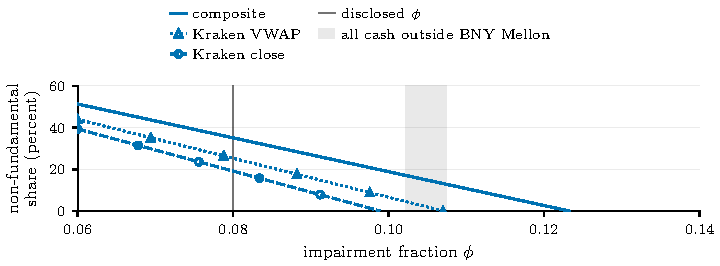
\includegraphics[width=\textwidth]{figs/fig_share_vs_phi.pdf}
\caption{Lower-edge non-fundamental share against impairment. Curves cross zero at one
minus their troughs. Shading treats cash outside BNY Mellon as impaired.}
\label{fig:share}
\end{figure}

Under (A1), $\phi$ is Circle's disclosed figure, and evaluating at $\rho=0$ uses the
lowest floor (A3) allows. Against the circulating supply at the trough, which exceeds
the \$40B figure Circle used, $\phi$ is $0.079$, below the headline $0.08$.

Circle's disclosure quantifies only the SVB deposit, but the same update itemizes the
whole cash leg: \$9.7B, of which \$5.4B sat at BNY Mellon, \$3.3B at SVB and \$1B at
Customers Bank, with no exposure to Silvergate~\cite{circle2023update}. With the \$32.4B
Treasury leg the same update reports, reserves total \$42.1B. Treating all cash outside
BNY Mellon as impaired gives $\phi=0.102$ on that total, where the
lower edge is $17.2\%$ on the composite and $4.7\%$ on Kraken's VWAP and Kraken's close
returns no verdict. On the \$40B base the same reading gives $\phi=0.1075$, where only
the composite still returns a verdict, at $12.8\%$.

Kraken's $240$ hourly bars run one day longer than the composite's $216$-hour window,
in which four snapshots are absent, and against that denominator its close breaches the
\$0.92 floor in 9 hours, its VWAP in 10, and its hourly low in 12. Sub-floor trades
themselves fall in twelve clock hours, $37{,}303$ of them worth \$154.0M.

Because the estimator needs only a price and a publicly quantified $\phi$, it can be
evaluated at every hour of the frozen window (Figure~\ref{fig:event}). Of USDC's $212$
in-window hourly readings, $9$ lie below the \$0.92 floor, and all nine fall on 11~March
2023 between 06{:}59 and 16{:}00~UTC, shaded in both panels. The
tenth hour of that window, at 08{:}57, recovers to \$0.9216. That impossibility window measures duration and
specificity. It adds no evidence volume, because hourly prices within one episode are
near-unit-root, with lag-1 autocorrelation $r=0.963$, so the $212$ readings carry an
AR(1)-adjusted effective sample size $n(1-r)/(1+r)=4.0$. The lower edge, $q^{\star}$, and the
floor-breach indicator are three readings of $1-P_{\mathrm{obs}}-\phi$, so their agreement
corroborates nothing.
